% Options for packages loaded elsewhere
\PassOptionsToPackage{unicode}{hyperref}
\PassOptionsToPackage{hyphens}{url}
%
\documentclass[
]{article}
\usepackage{lmodern}
\usepackage{amssymb,amsmath}
\usepackage{ifxetex,ifluatex}
\ifnum 0\ifxetex 1\fi\ifluatex 1\fi=0 % if pdftex
  \usepackage[T1]{fontenc}
  \usepackage[utf8]{inputenc}
  \usepackage{textcomp} % provide euro and other symbols
\else % if luatex or xetex
  \usepackage{unicode-math}
  \defaultfontfeatures{Scale=MatchLowercase}
  \defaultfontfeatures[\rmfamily]{Ligatures=TeX,Scale=1}
\fi
% Use upquote if available, for straight quotes in verbatim environments
\IfFileExists{upquote.sty}{\usepackage{upquote}}{}
\IfFileExists{microtype.sty}{% use microtype if available
  \usepackage[]{microtype}
  \UseMicrotypeSet[protrusion]{basicmath} % disable protrusion for tt fonts
}{}
\makeatletter
\@ifundefined{KOMAClassName}{% if non-KOMA class
  \IfFileExists{parskip.sty}{%
    \usepackage{parskip}
  }{% else
    \setlength{\parindent}{0pt}
    \setlength{\parskip}{6pt plus 2pt minus 1pt}}
}{% if KOMA class
  \KOMAoptions{parskip=half}}
\makeatother
\usepackage{xcolor}
\IfFileExists{xurl.sty}{\usepackage{xurl}}{} % add URL line breaks if available
\IfFileExists{bookmark.sty}{\usepackage{bookmark}}{\usepackage{hyperref}}
\hypersetup{
  pdftitle={Vertex Nomination via Seeded Graph Matching},
  pdfauthor={Carey E. Priebe, Youngser Park, Heather Patsolic, Vince Lyzinski   Johns Hopkins University},
  hidelinks,
  pdfcreator={LaTeX via pandoc}}
\urlstyle{same} % disable monospaced font for URLs
\usepackage[margin=1in]{geometry}
\usepackage{color}
\usepackage{fancyvrb}
\newcommand{\VerbBar}{|}
\newcommand{\VERB}{\Verb[commandchars=\\\{\}]}
\DefineVerbatimEnvironment{Highlighting}{Verbatim}{commandchars=\\\{\}}
% Add ',fontsize=\small' for more characters per line
\usepackage{framed}
\definecolor{shadecolor}{RGB}{248,248,248}
\newenvironment{Shaded}{\begin{snugshade}}{\end{snugshade}}
\newcommand{\AlertTok}[1]{\textcolor[rgb]{0.94,0.16,0.16}{#1}}
\newcommand{\AnnotationTok}[1]{\textcolor[rgb]{0.56,0.35,0.01}{\textbf{\textit{#1}}}}
\newcommand{\AttributeTok}[1]{\textcolor[rgb]{0.77,0.63,0.00}{#1}}
\newcommand{\BaseNTok}[1]{\textcolor[rgb]{0.00,0.00,0.81}{#1}}
\newcommand{\BuiltInTok}[1]{#1}
\newcommand{\CharTok}[1]{\textcolor[rgb]{0.31,0.60,0.02}{#1}}
\newcommand{\CommentTok}[1]{\textcolor[rgb]{0.56,0.35,0.01}{\textit{#1}}}
\newcommand{\CommentVarTok}[1]{\textcolor[rgb]{0.56,0.35,0.01}{\textbf{\textit{#1}}}}
\newcommand{\ConstantTok}[1]{\textcolor[rgb]{0.00,0.00,0.00}{#1}}
\newcommand{\ControlFlowTok}[1]{\textcolor[rgb]{0.13,0.29,0.53}{\textbf{#1}}}
\newcommand{\DataTypeTok}[1]{\textcolor[rgb]{0.13,0.29,0.53}{#1}}
\newcommand{\DecValTok}[1]{\textcolor[rgb]{0.00,0.00,0.81}{#1}}
\newcommand{\DocumentationTok}[1]{\textcolor[rgb]{0.56,0.35,0.01}{\textbf{\textit{#1}}}}
\newcommand{\ErrorTok}[1]{\textcolor[rgb]{0.64,0.00,0.00}{\textbf{#1}}}
\newcommand{\ExtensionTok}[1]{#1}
\newcommand{\FloatTok}[1]{\textcolor[rgb]{0.00,0.00,0.81}{#1}}
\newcommand{\FunctionTok}[1]{\textcolor[rgb]{0.00,0.00,0.00}{#1}}
\newcommand{\ImportTok}[1]{#1}
\newcommand{\InformationTok}[1]{\textcolor[rgb]{0.56,0.35,0.01}{\textbf{\textit{#1}}}}
\newcommand{\KeywordTok}[1]{\textcolor[rgb]{0.13,0.29,0.53}{\textbf{#1}}}
\newcommand{\NormalTok}[1]{#1}
\newcommand{\OperatorTok}[1]{\textcolor[rgb]{0.81,0.36,0.00}{\textbf{#1}}}
\newcommand{\OtherTok}[1]{\textcolor[rgb]{0.56,0.35,0.01}{#1}}
\newcommand{\PreprocessorTok}[1]{\textcolor[rgb]{0.56,0.35,0.01}{\textit{#1}}}
\newcommand{\RegionMarkerTok}[1]{#1}
\newcommand{\SpecialCharTok}[1]{\textcolor[rgb]{0.00,0.00,0.00}{#1}}
\newcommand{\SpecialStringTok}[1]{\textcolor[rgb]{0.31,0.60,0.02}{#1}}
\newcommand{\StringTok}[1]{\textcolor[rgb]{0.31,0.60,0.02}{#1}}
\newcommand{\VariableTok}[1]{\textcolor[rgb]{0.00,0.00,0.00}{#1}}
\newcommand{\VerbatimStringTok}[1]{\textcolor[rgb]{0.31,0.60,0.02}{#1}}
\newcommand{\WarningTok}[1]{\textcolor[rgb]{0.56,0.35,0.01}{\textbf{\textit{#1}}}}
\usepackage{longtable,booktabs}
% Correct order of tables after \paragraph or \subparagraph
\usepackage{etoolbox}
\makeatletter
\patchcmd\longtable{\par}{\if@noskipsec\mbox{}\fi\par}{}{}
\makeatother
% Allow footnotes in longtable head/foot
\IfFileExists{footnotehyper.sty}{\usepackage{footnotehyper}}{\usepackage{footnote}}
\makesavenoteenv{longtable}
\usepackage{graphicx,grffile}
\makeatletter
\def\maxwidth{\ifdim\Gin@nat@width>\linewidth\linewidth\else\Gin@nat@width\fi}
\def\maxheight{\ifdim\Gin@nat@height>\textheight\textheight\else\Gin@nat@height\fi}
\makeatother
% Scale images if necessary, so that they will not overflow the page
% margins by default, and it is still possible to overwrite the defaults
% using explicit options in \includegraphics[width, height, ...]{}
\setkeys{Gin}{width=\maxwidth,height=\maxheight,keepaspectratio}
% Set default figure placement to htbp
\makeatletter
\def\fps@figure{htbp}
\makeatother
\usepackage[normalem]{ulem}
% Avoid problems with \sout in headers with hyperref
\pdfstringdefDisableCommands{\renewcommand{\sout}{}}
\setlength{\emergencystretch}{3em} % prevent overfull lines
\providecommand{\tightlist}{%
  \setlength{\itemsep}{0pt}\setlength{\parskip}{0pt}}
\setcounter{secnumdepth}{5}

\title{Vertex Nomination via Seeded Graph Matching}
\author{Carey E. Priebe, Youngser Park, Heather Patsolic, Vince Lyzinski Johns
Hopkins University}
\date{2020-07-16}

\begin{document}
\maketitle

\hypertarget{background}{%
\section{Background}\label{background}}

\begin{itemize}
\tightlist
\item
  A short summary of the methodology is
  \href{http://www.cis.jhu.edu/~parky/XDATA/SGM/vnsgm_summary.pdf}{here}.
\item
  The latest draft of our paper is \sout{here} (unlinked for the future
  newer version).
\item
  The poster for \href{http://www.siam.org/meetings/ns16/}{SIAMNS16} is
  \href{http://www.cis.jhu.edu/~parky/XDATA/SGM/SIAM-NS16-VNSGM.pdf}{here}.
\item
  The slide set for
  \href{https://www.amstat.org/meetings/jsm/2016/}{JSM2016} is
  \href{http://www.cis.jhu.edu/~parky/XDATA/SGM/JSM2016-VNLNM.pdf}{here}.
\end{itemize}

Here we describe our approach to both the simulations and the
illustrative experiments, which allows the same code to be used to
address a real problem in anger (when we don't know any truth except the
VOI \(x\) and some seeds \(S \leftrightarrow S'\)).\\
If it's a simulation or illustrative experiment: (1) generate \(G\) and
\(G'\) with some shared vertices and some unshared vertices, or start
with real data \(G\) and \(G'\) with a collection of known shared
vertices and some unknown or unshared vertices, and (2) randomly pick
VOI \(x\) and some number of seeds \(S\leftrightarrow S'\) from amongst
the shared vertices; then embark on our procedure described below. If
it's a real problem, with given VOI \(x\) and some seeds
\(S \leftrightarrow S'\), then embark immediately on our procedure
described below.

\hypertarget{toy-example}{%
\section{Toy Example}\label{toy-example}}

\begin{quote}
\textbf{input}: \(G\), \(G'\), seedset \(S\leftrightarrow S'\) (pairs of
vertices one in \(G\) \& one in \(G'\)), \(x\) (vertex of interest in
\(G\)), \(h \leq \ell\).\\
\textbf{output}: list of (\texttt{candidate},\texttt{probability})
where\\
- \texttt{candidates} are non-seed vertices in \(G'\) and\\
- \texttt{probability} is for nomination as match for \(x\).
\end{quote}

This toy example follows these steps:

\begin{enumerate}
\def\labelenumi{\arabic{enumi}.}
\tightlist
\item
  build a pair of \(\rho\)-correlated RDPG random graphs, \(G(V,E)\) \&
  \(G'(V',E')\), where \(|V|=|V'|=30\)
\item
  remove the last \(5\) vertices from \(G'\) to make
  \(|V(G)| \geq |V(G')|\)
\item
  randomly pick VOI \(x\) and \(s\) seeds from amongst the shared
  vertices
\item
  find \(S_x\), all seeds in \(N_h(x)\) in \(G\), and matching \(S'_x\)
  in \(G'\), let \(s_x = |S_x| = |S'_x|\), if \(s_x=0\), then
  ``\texttt{impossible1}''
\item
  let \(C'_x = N_\ell(S'_x)\) be the \emph{candidates} for the match
  \(x'\) to the VOI \(x\) for \(\ell\geq h\), if \(x' \notin C'_x\),
  then ``\texttt{impossible2}''
\item
  find \(G_x = \Omega(N_\ell[S_x])\) and \(G'_x = \Omega(N_\ell[S'_x])\)
\item
  do \texttt{SGM}\((G_x, G'_x, S_x \leftrightarrow S'_x)\) which returns
  \(P=|V_x| \times |V'_x|\) matching probability matrix
\item
  find \(\hat{x}' = \arg\max_{v \in {C'_x}} P[x,v]\)
\end{enumerate}

So now we do \texttt{SGM}\((G_x,G'_x,S_x \leftrightarrow S'_x)\) -- a
smaller SGM problem. (NB: original is this with \(h=\infty\).)

NB: Steps 4-8 are the same for simulation, illustrative experiment, and
real application.

\begin{Shaded}
\begin{Highlighting}[]
\KeywordTok{suppressMessages}\NormalTok{(}\KeywordTok{require}\NormalTok{(VN)) }
\KeywordTok{suppressMessages}\NormalTok{(}\KeywordTok{require}\NormalTok{(igraph))}

\NormalTok{sim <-}\StringTok{ }\OtherTok{TRUE} \CommentTok{# if TRUE, run simulation, otherwise do the HS experiment}
\NormalTok{HS <-}\StringTok{ "full"} \CommentTok{# or "core"}

\CommentTok{# parameters for finding seeds}
\NormalTok{s <-}\StringTok{ }\KeywordTok{ifelse}\NormalTok{(sim,}\DecValTok{4}\NormalTok{,}\DecValTok{12}\NormalTok{) }\CommentTok{# number of seeds to be used for SGM}
\NormalTok{h <-}\StringTok{ }\NormalTok{ell <-}\StringTok{ }\DecValTok{1} \CommentTok{# max walk for finding neighborhoods}

\CommentTok{# parameters for SGM}
\NormalTok{R <-}\StringTok{ }\DecValTok{100}     \CommentTok{# repeat SGM R times to get averaged P matrix}
\NormalTok{gamma <-}\StringTok{ }\FloatTok{0.1} \CommentTok{# number of iterations for the Frank-Wolfe algorithm}

\NormalTok{mc <-}\StringTok{ }\DecValTok{2}
\KeywordTok{set.seed}\NormalTok{(}\DecValTok{1234}\OperatorTok{+}\NormalTok{mc)}

\ControlFlowTok{if}\NormalTok{ (sim) \{}
    \CommentTok{# generate a pair of correlated graphs}
\NormalTok{    m <-}\StringTok{ }\DecValTok{5}  \CommentTok{# |J| = junk on G1}
\NormalTok{    n <-}\StringTok{ }\DecValTok{20} \CommentTok{# |W| = shared vertices on G1, not including x and S}
\NormalTok{    mp <-}\StringTok{ }\DecValTok{0} \CommentTok{# |J'| = junk on G2 }
\NormalTok{    d <-}\StringTok{ }\DecValTok{5}  \CommentTok{# for RDPG, dimension of the random vectors}
\NormalTok{    corr <-}\StringTok{ }\FloatTok{0.5} \CommentTok{# for correlated graphs}

\NormalTok{    (nV1 <-}\StringTok{ }\DecValTok{1}\OperatorTok{+}\NormalTok{s}\OperatorTok{+}\NormalTok{n}\OperatorTok{+}\NormalTok{m)}
\NormalTok{    (nV2 <-}\StringTok{ }\DecValTok{1}\OperatorTok{+}\NormalTok{s}\OperatorTok{+}\NormalTok{n}\OperatorTok{+}\NormalTok{mp)}
\NormalTok{    lpvs <-}\StringTok{ }\KeywordTok{sample_sphere_surface}\NormalTok{(}\DataTypeTok{dim=}\NormalTok{d, }\DataTypeTok{n=}\NormalTok{nV1)}\OperatorTok{/}\FloatTok{1.5} \CommentTok{# random vectors for RDPG}
\NormalTok{    gg <-}\StringTok{ }\KeywordTok{rdpg.sample.correlated}\NormalTok{(}\KeywordTok{t}\NormalTok{(lpvs),corr)}
\NormalTok{    g1 <-}\StringTok{ }\NormalTok{gg[[}\DecValTok{1}\NormalTok{]]; }
\NormalTok{    g2 <-}\StringTok{ }\NormalTok{gg[[}\DecValTok{2}\NormalTok{]]; }
\NormalTok{    g2 <-}\StringTok{ }\KeywordTok{delete_vertices}\NormalTok{(g2,}\DataTypeTok{v=}\NormalTok{(nV2}\OperatorTok{+}\DecValTok{1}\NormalTok{)}\OperatorTok{:}\NormalTok{nV1); }\CommentTok{# remove m vertices from G' to make |V(G)| != |V(G')|}
\NormalTok{    W <-}\StringTok{ }\KeywordTok{intersect}\NormalTok{(}\KeywordTok{V}\NormalTok{(g1),}\KeywordTok{V}\NormalTok{(g2)) }\CommentTok{# shared vertices}
\NormalTok{\} }\ControlFlowTok{else}\NormalTok{ \{}
    \KeywordTok{data}\NormalTok{(}\StringTok{"HSgraphs"}\NormalTok{)}
    \ControlFlowTok{if}\NormalTok{ (HS }\OperatorTok{==}\StringTok{ "full"}\NormalTok{) \{}
        \CommentTok{# rearrange the vertices so that the to-be-selected seeds are valid}
\NormalTok{        perm.fb <-}\StringTok{ }\KeywordTok{c}\NormalTok{(coremap[,}\DecValTok{1}\NormalTok{],}\KeywordTok{setdiff}\NormalTok{(}\DecValTok{1}\OperatorTok{:}\KeywordTok{vcount}\NormalTok{(HSfbgraphfull),coremap[,}\DecValTok{1}\NormalTok{]))}
\NormalTok{        perm.fr <-}\StringTok{ }\KeywordTok{c}\NormalTok{(coremap[,}\DecValTok{2}\NormalTok{],}\KeywordTok{setdiff}\NormalTok{(}\DecValTok{1}\OperatorTok{:}\KeywordTok{vcount}\NormalTok{(HSfriendsgraphfull),coremap[,}\DecValTok{2}\NormalTok{]))}
\NormalTok{        g1 <-}\StringTok{ }\KeywordTok{permute.vertices}\NormalTok{(HSfbgraphfull,perm.fb) }\CommentTok{# (156,1437)}
\NormalTok{        g2 <-}\StringTok{ }\KeywordTok{permute.vertices}\NormalTok{(HSfriendsgraphfull,perm.fr) }\CommentTok{# (134,668)}
\NormalTok{        W <-}\StringTok{ }\DecValTok{1}\OperatorTok{:}\KeywordTok{nrow}\NormalTok{(coremap) }\CommentTok{# seeds should be selected from the shared (core) vertices}
\NormalTok{    \} }\ControlFlowTok{else}\NormalTok{ \{ }\CommentTok{# core graphs}
\NormalTok{        g1 <-}\StringTok{ }\NormalTok{HSfbgraphcore }\CommentTok{# (82,513)}
\NormalTok{        g2 <-}\StringTok{ }\NormalTok{HSfrgraphcore }\CommentTok{# (82,214)}
\NormalTok{        W <-}\StringTok{ }\KeywordTok{intersect}\NormalTok{(}\KeywordTok{V}\NormalTok{(g1),}\KeywordTok{V}\NormalTok{(g2)) }\CommentTok{# shared vertices}
\NormalTok{    \}}
\NormalTok{\}}
\end{Highlighting}
\end{Shaded}

\begin{Shaded}
\begin{Highlighting}[]
\CommentTok{# Randomly select x and S from W, the shared vertices}
\CommentTok{#NB: Somehow, I cannot reproduce the previous demo in the vignette, so I hard coded!}
\NormalTok{(x <-}\StringTok{ }\DecValTok{22}\NormalTok{) }\CommentTok{#sample(W,1))}
\end{Highlighting}
\end{Shaded}

\begin{verbatim}
# [1] 22
\end{verbatim}

\begin{Shaded}
\begin{Highlighting}[]
\NormalTok{W <-}\StringTok{ }\KeywordTok{setdiff}\NormalTok{(W,x) }\CommentTok{# exclude x from W}
\NormalTok{maxseed <-}\StringTok{ }\KeywordTok{min}\NormalTok{(}\KeywordTok{length}\NormalTok{(W),s)}
\NormalTok{(S <-}\StringTok{ }\KeywordTok{c}\NormalTok{(}\DecValTok{1}\NormalTok{,}\DecValTok{8}\NormalTok{,}\DecValTok{18}\NormalTok{,}\DecValTok{25}\NormalTok{)) }\CommentTok{#sort(sample(W,maxseed))) }
\end{Highlighting}
\end{Shaded}

\begin{verbatim}
# [1]  1  8 18 25
\end{verbatim}

\begin{Shaded}
\begin{Highlighting}[]
\CommentTok{# Determine Sx and C'x, then do SGM}
\NormalTok{NBDS <-}\StringTok{ }\KeywordTok{vnsgm.ordered}\NormalTok{(x,S,g1,g2,h,ell,R,gamma,}\DataTypeTok{plotF=}\OtherTok{TRUE}\NormalTok{)}
\end{Highlighting}
\end{Shaded}

\begin{figure}
\centering
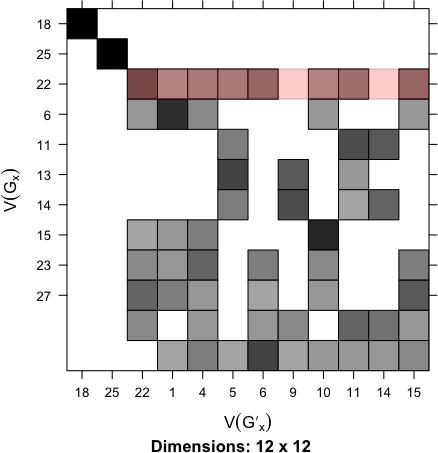
\includegraphics{vn_files/figure-latex/sgm-1.png}
\caption{A submatrix of a probability matrix output from SGM. Rows
correspond to vertices in \(V(G_x)\) and columns correspond to vertices
in \(V(G'_x)\). The first 2 rows and columns correspond to the seeds
\((S_x,S'_x)\), The next row is \(x\). The shaded area (in pink) depicts
matching probabilities of vertices in \(C'_x\) against \(x\) in
\(V(G_x)\). The vertices with the highest probability among these
\emph{candidates} is nominated as our best guess for \(x'\).}
\end{figure}

\begin{Shaded}
\begin{Highlighting}[]
\KeywordTok{str}\NormalTok{(NBDS)}
\end{Highlighting}
\end{Shaded}

\begin{verbatim}
# List of 9
#  $ case     : chr "possible"
#  $ x        : num 22
#  $ S        : num [1:4] 1 8 18 25
#  $ Sx       : num [1:2] 18 25
#  $ Sxp      : num [1:2] 18 25
#  $ Cxp      : int [1:10] 1 4 5 6 9 10 11 14 15 22
#  $ labelsGx : num [1:10] 18 25 22 6 11 13 14 15 23 27
#  $ labelsGxp: num [1:12] 18 25 22 1 4 5 6 9 10 11 ...
#  $ P        : num [1:12, 1:12] 1 0 0 0 0 0 0 0 0 0 ...
\end{verbatim}

\begin{Shaded}
\begin{Highlighting}[]
\CommentTok{# Determine x' amongst the candidates based on the matching probability from SGM}
\NormalTok{Sx <-}\StringTok{ }\NormalTok{NBDS}\OperatorTok{$}\NormalTok{Sx}
\NormalTok{x <-}\StringTok{ }\NormalTok{NBDS}\OperatorTok{$}\NormalTok{labelsGxp[}\KeywordTok{length}\NormalTok{(Sx)}\OperatorTok{+}\DecValTok{1}\NormalTok{]}
\NormalTok{x.ind <-}\StringTok{ }\KeywordTok{which}\NormalTok{(NBDS}\OperatorTok{$}\NormalTok{labelsGx}\OperatorTok{==}\NormalTok{x)}
\NormalTok{Cxp <-}\StringTok{ }\KeywordTok{match}\NormalTok{(NBDS}\OperatorTok{$}\NormalTok{Cxp,NBDS}\OperatorTok{$}\NormalTok{labelsGxp) }

\ControlFlowTok{if}\NormalTok{ (NBDS}\OperatorTok{$}\NormalTok{case}\OperatorTok{==}\StringTok{"possible"}\NormalTok{) \{}
\NormalTok{    prob <-}\StringTok{ }\NormalTok{NBDS}\OperatorTok{$}\NormalTok{P[x.ind,Cxp]}
    \KeywordTok{names}\NormalTok{(prob) <-}\StringTok{ }\NormalTok{NBDS}\OperatorTok{$}\NormalTok{labelsGxp[Cxp]}
\NormalTok{    x.prob <-}\StringTok{ }\NormalTok{prob[}\KeywordTok{which.max}\NormalTok{(prob)]}
\NormalTok{    vhatstar <-}\StringTok{ }\KeywordTok{as.integer}\NormalTok{(}\KeywordTok{names}\NormalTok{(x.prob))}
\NormalTok{    rank.prob <-}\StringTok{ }\KeywordTok{rank}\NormalTok{(}\OperatorTok{-}\NormalTok{prob,}\DataTypeTok{ties.method =} \StringTok{"average"}\NormalTok{)}
    \KeywordTok{plot}\NormalTok{(}\KeywordTok{as.integer}\NormalTok{(}\KeywordTok{names}\NormalTok{(prob)), prob, }\DataTypeTok{type=}\StringTok{"h"}\NormalTok{,}\DataTypeTok{col=}\DecValTok{2}\NormalTok{, }\DataTypeTok{lwd=}\DecValTok{2}\NormalTok{)}
\NormalTok{    rank.prob <-}\StringTok{ }\KeywordTok{matrix}\NormalTok{(rank.prob,}\DataTypeTok{nrow=}\DecValTok{1}\NormalTok{); }\KeywordTok{colnames}\NormalTok{(rank.prob) <-}\StringTok{ }\KeywordTok{paste0}\NormalTok{(}\StringTok{"V"}\NormalTok{,}\KeywordTok{names}\NormalTok{(prob))}
    \KeywordTok{kable}\NormalTok{(rank.prob,}\DataTypeTok{caption=}\StringTok{"Rank of matching probability for candidates"}\NormalTok{)}
\NormalTok{\}}
\end{Highlighting}
\end{Shaded}

\begin{figure}
\centering
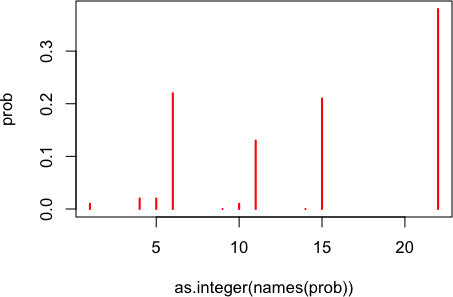
\includegraphics{vn_files/figure-latex/prob-1.png}
\caption{A bar plot of the matching probability of the candidates. The
vertex 22 in \(G'_x\) has the highest probability so is nominated as
\(x'\).}
\end{figure}

\begin{longtable}[]{@{}rrrrrrrrrr@{}}
\caption{Rank of matching probability for candidates}\tabularnewline
\toprule
V1 & V4 & V5 & V6 & V9 & V10 & V11 & V14 & V15 & V22\tabularnewline
\midrule
\endfirsthead
\toprule
V1 & V4 & V5 & V6 & V9 & V10 & V11 & V14 & V15 & V22\tabularnewline
\midrule
\endhead
7.5 & 5.5 & 5.5 & 2 & 9.5 & 7.5 & 4 & 9.5 & 3 & 1\tabularnewline
\bottomrule
\end{longtable}

\begin{figure}
\centering
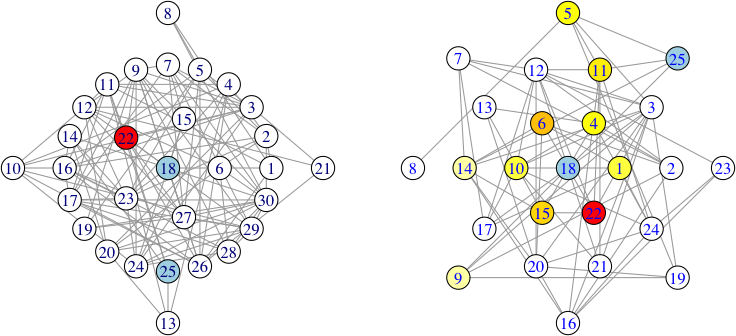
\includegraphics{vn_files/figure-latex/plotg3-1.png}
\caption{Plot of \(G\) (left) and \(G'\) (right), where the vertices are
colored by red in \(G\): \(x\), cyan on both graphs: \(S_x\),
\texttt{heat.colors} in \(G'\): candidates (the more red the color is,
the higher the rank of the candidate is). In both graphs, the center
vertex is one of the seeds in \(S_x\), its first neighbors are in the
first ring, their first neighbors are in the next ring, and the rest are
placed in the outmost ring.}
\end{figure}

\hypertarget{simulation}{%
\section{Simulation}\label{simulation}}

We repeat the above 1000 times by generating new graphs each time, as
well as new \(x\) and \(S\).

We define the normalized rank of the VOI \(x\) in \(G'\) with respect to
the size of the candidate list \(C'_x\) as follows,

\[normalized~rank = \frac{rank(x') -1}{|C'_x|-1},\]

so that values of 0, 0.5, and 1 imply that the VOI is first, half-way
down, and last in the candidate list, respectively.

NB: In the tables and plots below,

\begin{itemize}
\tightlist
\item
  \texttt{s1} means the number of seeds for \texttt{SGM}, \(s_x=1\) and
  so on.
\item
  \texttt{mean.ncand} means averaged number of candidates for each case.
\item
  \texttt{mean.nrank} means averaged normalized rank for each case.
\end{itemize}

\begin{longtable}[]{@{}llrrr@{}}
\caption{A summary of the simulation for
\texttt{corr=0.1}}\tabularnewline
\toprule
case & seed & count & mean.ncand & mean.nrank\tabularnewline
\midrule
\endfirsthead
\toprule
case & seed & count & mean.ncand & mean.nrank\tabularnewline
\midrule
\endhead
impossible1 & s0 & 232 & 0.0 & NA\tabularnewline
impossible2 & s0 & 365 & 8.8 & NA\tabularnewline
possible & s1 & 164 & 8.3 & 0.46\tabularnewline
possible & s2 & 168 & 12.7 & 0.47\tabularnewline
possible & s3 & 67 & 15.5 & 0.42\tabularnewline
possible & s4 & 4 & 16.0 & 0.36\tabularnewline
\bottomrule
\end{longtable}

\begin{longtable}[]{@{}llrrr@{}}
\caption{A summary of the simulation for
\texttt{corr=0.9}}\tabularnewline
\toprule
case & seed & count & mean.ncand & mean.nrank\tabularnewline
\midrule
\endfirsthead
\toprule
case & seed & count & mean.ncand & mean.nrank\tabularnewline
\midrule
\endhead
impossible1 & s0 & 198 & 0.0 & NaN\tabularnewline
impossible2 & s0 & 32 & 7.6 & NaN\tabularnewline
possible & s1 & 389 & 8.4 & 0.17\tabularnewline
possible & s2 & 290 & 12.7 & 0.03\tabularnewline
possible & s3 & 82 & 15.3 & 0.01\tabularnewline
possible & s4 & 9 & 15.8 & 0.00\tabularnewline
\bottomrule
\end{longtable}

\hypertarget{number-of-candidates}{%
\subsection{Number of candidates?}\label{number-of-candidates}}

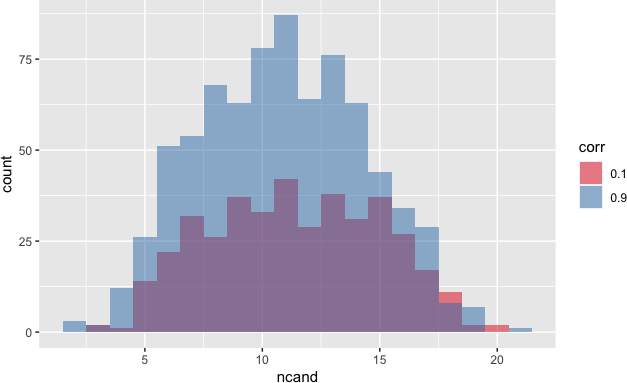
\includegraphics{vn_files/figure-latex/cand-1.png}
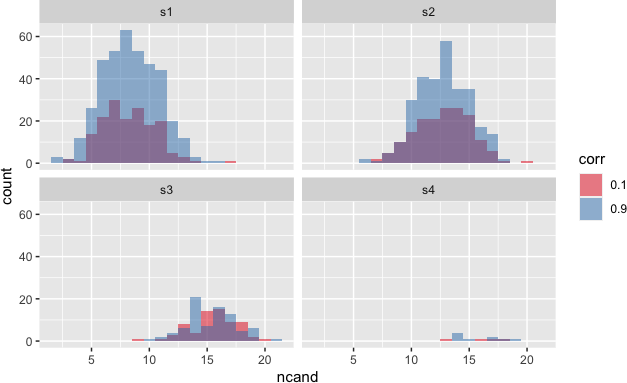
\includegraphics{vn_files/figure-latex/ncand-1.png}

\hypertarget{rank-of-x}{%
\subsection{\texorpdfstring{Rank of
\(x'\)?}{Rank of x'?}}\label{rank-of-x}}

\begin{figure}
\centering
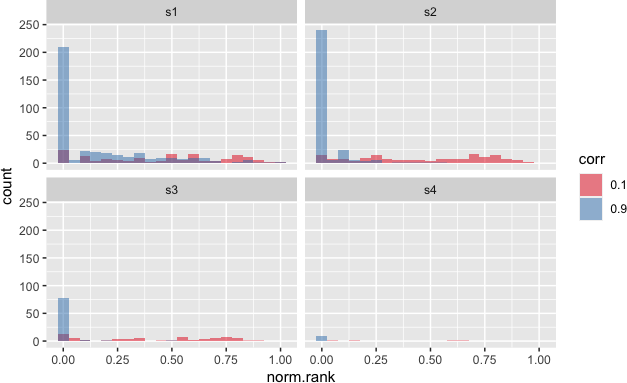
\includegraphics{vn_files/figure-latex/rank-1.png}
\caption{A histogram of the normalized rank of \(x'\) as a function of
the number of seeds \(s_x\).}
\end{figure}

\begin{figure}
\centering
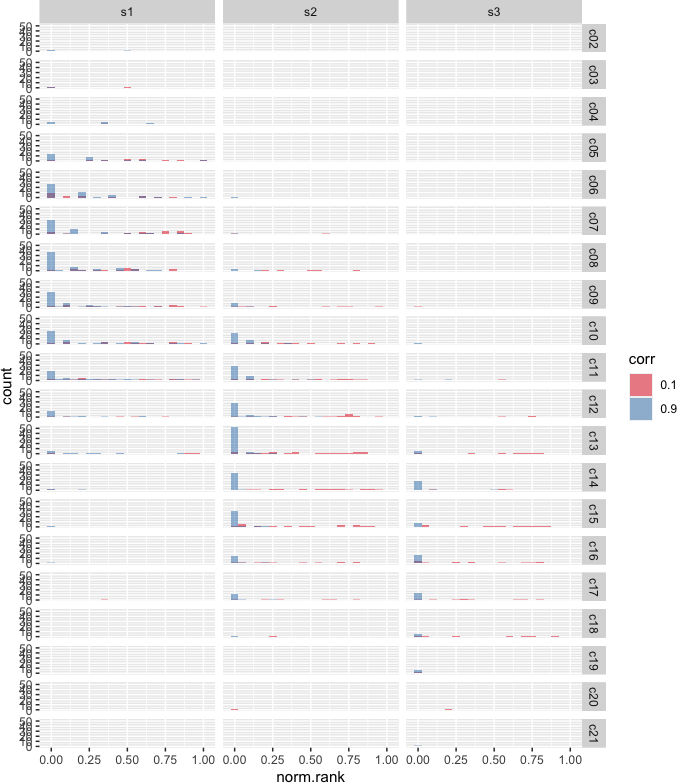
\includegraphics{vn_files/figure-latex/rank2-1.png}
\caption{A histogram of the normalized rank of \(x'\) as a function of
the number of candidates and the number of seeds.}
\end{figure}

\hypertarget{real-data}{%
\section{Real Data}\label{real-data}}

\begin{quote}
R. Mastrandrea, J. Fournet, and A. Barrat, \emph{Contact patterns in a
high school: a comparison between data collected using wearable sensors,
contact diaries and friendship surveys}, PLoS ONE, 2015.
\end{quote}

We look at two High School friendship networks on over-lapping vertex
sets found in our draft. The first network consists of 134 vertices,
each representing a particular student, in which two vertices are
adjacent if one of the students reported or a survey that the two are
friends. The second network, with 156 vertices, consists of a Facebook
network of profiles in which two vertices are adjacent if they were
friends on Facebook. There are 82 \(core\) vertices across the two
networks for which we know the bijection between the two vertex sets,
and it is known that no such bijection exists among the remaining
vertices.

\hypertarget{full-graphs}{%
\subsection{Full Graphs}\label{full-graphs}}

First, we do the same experiment as above using the full graphs. We
randomly select the VOI \(x\) and seeds \(S\) from the shared vertices
(82 core vertices) and repeat for \(MC=1000\) times. Since we are
choosing the VOI and seeds to be in the core vertex sets, the VOI will
exist in the second network; it just may not exist in \(C_x'\) (the
candidate set generated by the seeds) -- i.e.~while the VOI \(x\) is
guaranteed to have a match \(x'\), this vertex will not be found if it
is not also in \(C'_x\) (\texttt{impossible2}).

\begin{longtable}[]{@{}llrrr@{}}
\caption{A summary statistics using the full graphs}\tabularnewline
\toprule
case & seed & count & mean.ncand & mean.nrank\tabularnewline
\midrule
\endfirsthead
\toprule
case & seed & count & mean.ncand & mean.nrank\tabularnewline
\midrule
\endhead
impossible1 & s0 & 230 & 0.0 & NaN\tabularnewline
impossible2 & s0 & 688 & 12.8 & NaN\tabularnewline
possible & s01 & 11 & 7.9 & 0.69\tabularnewline
possible & s02 & 27 & 13.1 & 0.44\tabularnewline
possible & s03 & 15 & 20.1 & 0.51\tabularnewline
possible & s04 & 15 & 23.5 & 0.51\tabularnewline
possible & s05 & 9 & 28.7 & 0.51\tabularnewline
possible & s06 & 3 & 36.0 & 0.51\tabularnewline
possible & s07 & 1 & 35.0 & 0.50\tabularnewline
possible & s09 & 1 & 33.0 & 0.50\tabularnewline
\bottomrule
\end{longtable}

\hypertarget{number-of-candidates-1}{%
\subsubsection{Number of candidates?}\label{number-of-candidates-1}}

\begin{figure}
\centering
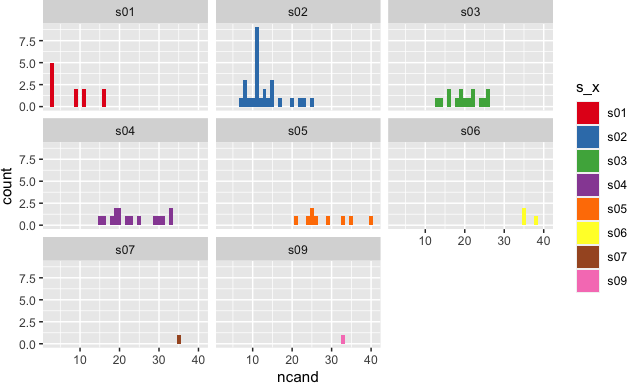
\includegraphics{vn_files/figure-latex/cand2-1.png}
\caption{A histogram of the number of candidates as a function of the
number of seeds.}
\end{figure}

\hypertarget{rank-of-x-1}{%
\subsubsection{\texorpdfstring{Rank of
\(x'\)?}{Rank of x'?}}\label{rank-of-x-1}}

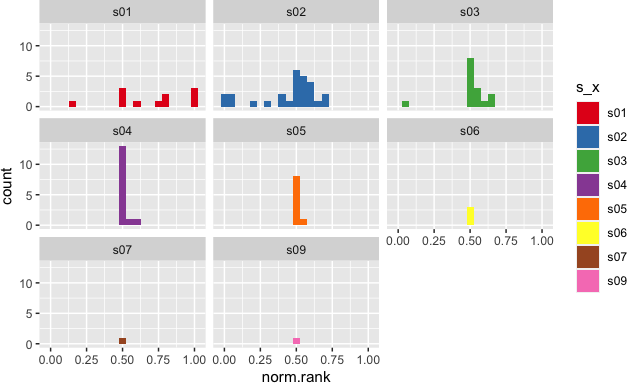
\includegraphics{vn_files/figure-latex/rank3-1.png}
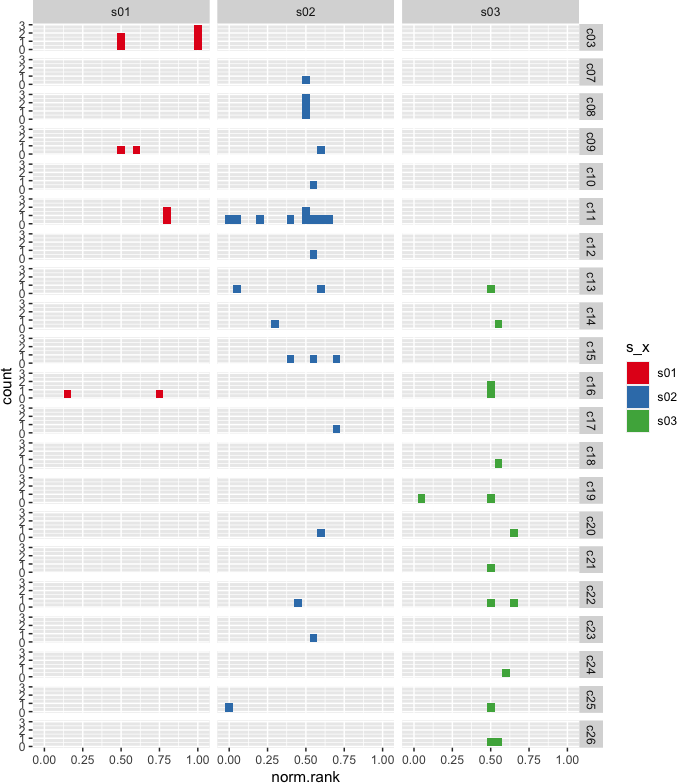
\includegraphics{vn_files/figure-latex/rank4-1.png}

\hypertarget{core-graphs}{%
\subsection{Core Graphs}\label{core-graphs}}

We do the same experiment as above using only the core graphs. We
randomly select the VOI \(x\) and seeds \(S\) from the shared vertices
(82 core vertices) and repeat for \(MC=1000\) times.

\begin{longtable}[]{@{}llrrrrr@{}}
\caption{A summary statistics using the core graphs}\tabularnewline
\toprule
case & seed & count & mean.ncand & mean.nrank & \#pvals\textless0.05 &
mean(nrank{[}pval\textless0.05{]})\tabularnewline
\midrule
\endfirsthead
\toprule
case & seed & count & mean.ncand & mean.nrank & \#pvals\textless0.05 &
mean(nrank{[}pval\textless0.05{]})\tabularnewline
\midrule
\endhead
impossible1 & s0 & 207 & 0.0 & NaN & 0 & NaN\tabularnewline
impossible2 & s0 & 283 & 8.6 & NaN & 0 & NaN\tabularnewline
possible & s1 & 99 & 6.4 & 0.42 & 40 & 0.15\tabularnewline
possible & s2 & 150 & 10.9 & 0.34 & 55 & 0.19\tabularnewline
possible & s3 & 138 & 14.3 & 0.35 & 48 & 0.21\tabularnewline
possible & s4 & 65 & 15.4 & 0.36 & 42 & 0.32\tabularnewline
possible & s5 & 39 & 17.6 & 0.41 & 31 & 0.41\tabularnewline
possible & s6 & 17 & 20.4 & 0.36 & 12 & 0.38\tabularnewline
possible & s7 & 1 & 20.0 & 0.16 & 0 & NaN\tabularnewline
possible & s8 & 1 & 21.0 & 0.50 & 1 & 0.50\tabularnewline
\bottomrule
\end{longtable}

\begin{figure}
\centering
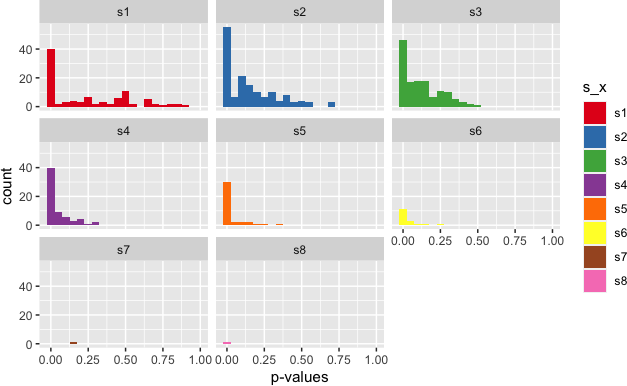
\includegraphics{vn_files/figure-latex/pval-1.png}
\caption{A density of the p-values as a function of the number of
seeds.}
\end{figure}

\hypertarget{number-of-candidates-2}{%
\subsubsection{Number of candidates?}\label{number-of-candidates-2}}

\begin{figure}
\centering
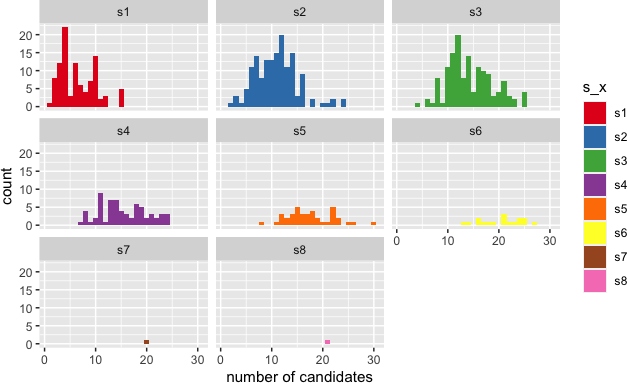
\includegraphics{vn_files/figure-latex/ccand2-1.png}
\caption{A histogram of the number of candidates as a function of the
number of seeds.}
\end{figure}

\hypertarget{rank-of-x-2}{%
\subsubsection{\texorpdfstring{Rank of
\(x'\)?}{Rank of x'?}}\label{rank-of-x-2}}

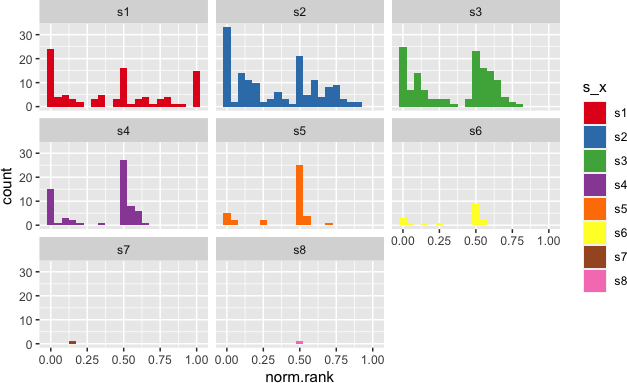
\includegraphics{vn_files/figure-latex/crank3-1.png}
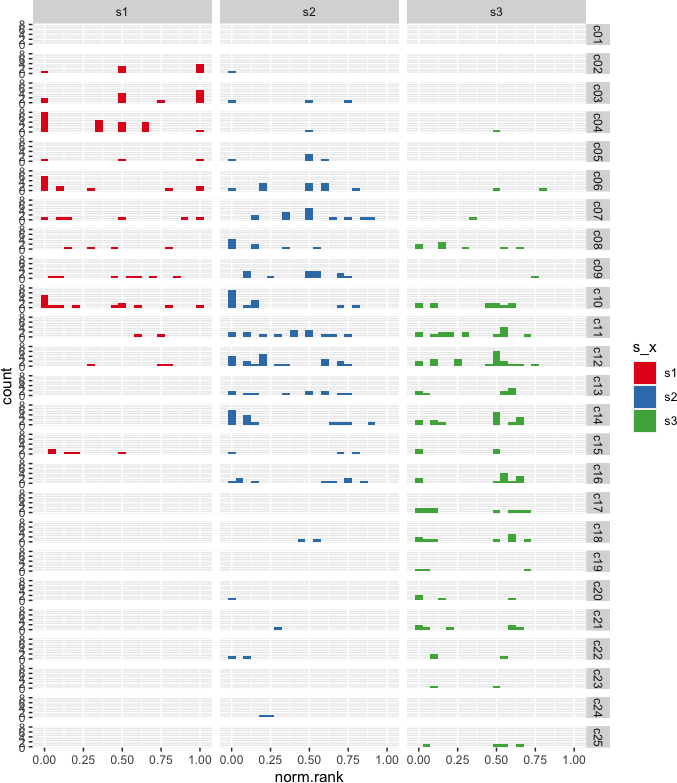
\includegraphics{vn_files/figure-latex/crank4-1.png}

\end{document}
